\documentclass{beamer}
\usepackage[T2A]{fontenc}
\usepackage[utf8]{inputenc}
\usepackage[russian]{babel}
\usepackage[style=authortitle,backend=bibtex]{biblatex}
\usefonttheme[onlymath]{serif}
\addbibresource{refs.bib}
%\usetheme{Boadilla}
\usetheme[numbers, totalnumbers, minimal, nologo]{Boadilla}
\setbeamertemplate{sidebar right}{}
\setbeamertemplate{footline}
{
  \leavevmode%
  \hbox{%
  \begin{beamercolorbox}[wd=.333333\paperwidth,ht=2.25ex,dp=1ex,center]{author in head/foot}%
    \usebeamerfont{author in head/foot}\insertauthor
  \end{beamercolorbox}%
  \begin{beamercolorbox}[wd=.333333\paperwidth,ht=2.25ex,dp=1ex,center]{title in head/foot}%
    \usebeamerfont{title in head/foot}\inserttitle
  \end{beamercolorbox}%
  \begin{beamercolorbox}[wd=.333333\paperwidth,ht=2.25ex,dp=1ex,right]{date in head/foot}%
    \usebeamerfont{date in head/foot}\insertshortdate{}\hspace*{2em}
    \insertframenumber{} / \inserttotalframenumber\hspace*{2ex} 
  \end{beamercolorbox}}%
  \vskip0pt%
}
\usepackage{graphicx} % Required for inserting images

\usepackage[T2A]{fontenc}
\usepackage[utf8]{inputenc}

\title{Введение в компьютерную графику. Занятие 1}
\author{Кедров A.A.}
\institute{Математическое моделирование (на английском языке)}
\date{\today}

\begin{document}

\begin{frame}
\titlepage
\end{frame}

\begin{frame}{Содержание}
    \tableofcontents
\end{frame}

\section{3D-рендеринг}

\begin{frame}
\frametitle{3D-рендеринг}
\begin{alertblock}{Определение} 
\alert{Рендеринг} --- это процесесс создания изображения на основе имеющейся модели.
\end{alertblock}

Под \alert{3D-рендерингом} обычно подразумевают процесс проецирования 3-х мерной модели на 2-х мерное изображение.

\begin{figure}
\centering
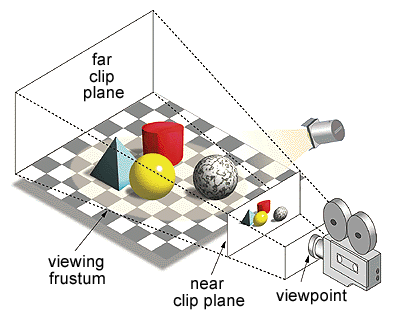
\includegraphics[width=0.45\textwidth]{3d-graphics.png}
\end{figure}

\end{frame}

\begin{frame}{Разновидности 3D-рендеринга}
Основные алгоритмы 3D-рендеринга:
\begin{itemize}
    \item Растреризация (rasterization)
    \item Трассировка лучей (ray-tracing)
\end{itemize}

Виды рендеринга по типу используемых устройств:
\begin{itemize}
    \item Software (все расчёты идут на CPU)
    \item Hardware/Accelerated (используют GPU/ускорители вычислений)
\end{itemize}

\begin{figure}
\centering
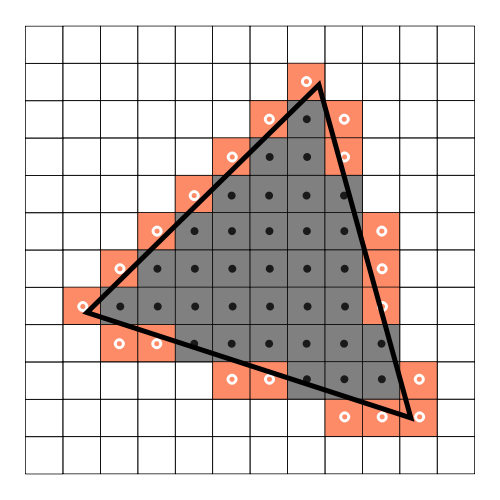
\includegraphics[height=0.30\textwidth]{rasterization.jpg}
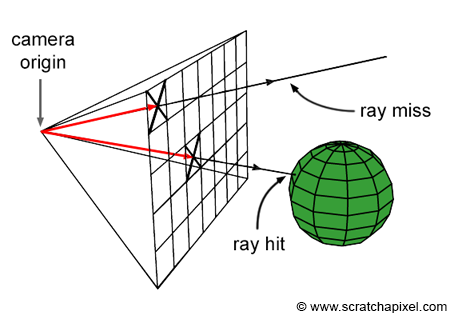
\includegraphics[height=0.30\textwidth]{rt-setup2.png}
\caption{Растреризация треугальника (слева). Трассировка лучей из камеры наблюдения (справа)}
\end{figure}

\end{frame}

\section{Аффинное пространство}
\begin{frame}
\frametitle{Базовые линейные преобразования объектами}
\begin{itemize}
    \item Вращение 
        \begin{equation*}
            M_z(\alpha) = \left[\begin{matrix}
                \cos(\alpha)  &-\sin(\alpha) &0 \\
                \sin(\alpha) \ &\cos(\alpha)   &0 \\
                0          &0            &1
            \end{matrix} \right]
        \end{equation*}
    \item Масштабирование
        \begin{equation*}
            M(s_x, s_y, s_z) = \left[\begin{matrix}
                s_x  & 0  &0 \\
                0 &s_y &0 \\
                0  &0 &s_z
            \end{matrix} \right]
        \end{equation*}
    \item Перемещение
        \begin{equation*}
            M(\vec{b}) = ?
        \end{equation*}
\end{itemize}
\begin{block} {Проблема}
Нет линейного преобразования $M$, такого что $M(\vec{b})\cdot \vec{a} = \vec{a} + \vec{b}$ для любого $\vec{a}$
\end{block}

\end{frame}

\begin{frame}
\frametitle{Аффинное пространство}
\begin{alertblock}{Определение}
Аффинное пространство --- это \emph{множество точек} $A$, \emph{векторное пространство} $\vec{A}$ и \emph{действие аддитивной группы} $\vec{A}$ над множеством $A$
\end{alertblock}
\begin{equation*}
    A \times \vec{A} \rightarrow A
\end{equation*}
Со следующими свойствами:
\begin{itemize}
    \item Идентичность
        \begin{equation*}
            a + \vec{0} = a
        \end{equation*}
    \item Ассоциативность
        \begin{equation*}
            (a + \vec{v}) + \vec{w} = a + (\vec{v} + \vec{w}) 
        \end{equation*}
    \item Можно определить операцию вычитания
        \begin{equation*}
            \forall a, b \ \exists! \, \vec{v} = b - a: a + \vec{v} = b
        \end{equation*}
\end{itemize}
\end{frame}

\begin{frame}
\frametitle{Аффинные преобразования}
Аффинные преобразования над аффинным пространством можно представить следующим образом:
\begin{equation*}
    f(x) = Ax + \vec{b}
\end{equation*}
где $A$ --- линейное преобразование над точкой $x$

В компьютерной графике используется представление через дополненные матрицы.

\begin{equation*}
    x \rightarrow \textbf{X} = \left[\begin{matrix}
        x_1 \\
        x_2 \\
        x_3 \\
        1
    \end{matrix}\right] \quad f(x) = \textbf{M} = \left[\begin{matrix}
        A_{11} & A_{12} & A_{13} & b_1 \\
        A_{11} & A_{12} & A_{13} & b_2 \\
        A_{11} & A_{12} & A_{13} & b_3 \\
        0      & 0      & 0      & 1
    \end{matrix}\right] \quad f(x) \rightarrow \textbf{M} \textbf{X}
\end{equation*}
\begin{block}{Замечание}
    Данное представление удобно тем, что может быть использовано и для векторов. $\vec{x} \rightarrow \vec{\textbf{X}} = \left[x_1, x_2, x_3, 0\right]^T$. Тогда $\textbf{M}\vec{\textbf{X}} \leftarrow A \vec{x}$
\end{block}
\end{frame}

\section{Гомогенные координаты}
\begin{frame}{Проекции разных объектов в перспективе}
    \begin{itemize}
        \item Куб. Грани одинаковых размеров выглядят по-разному в перспективе
        \begin{figure}
            \centering
            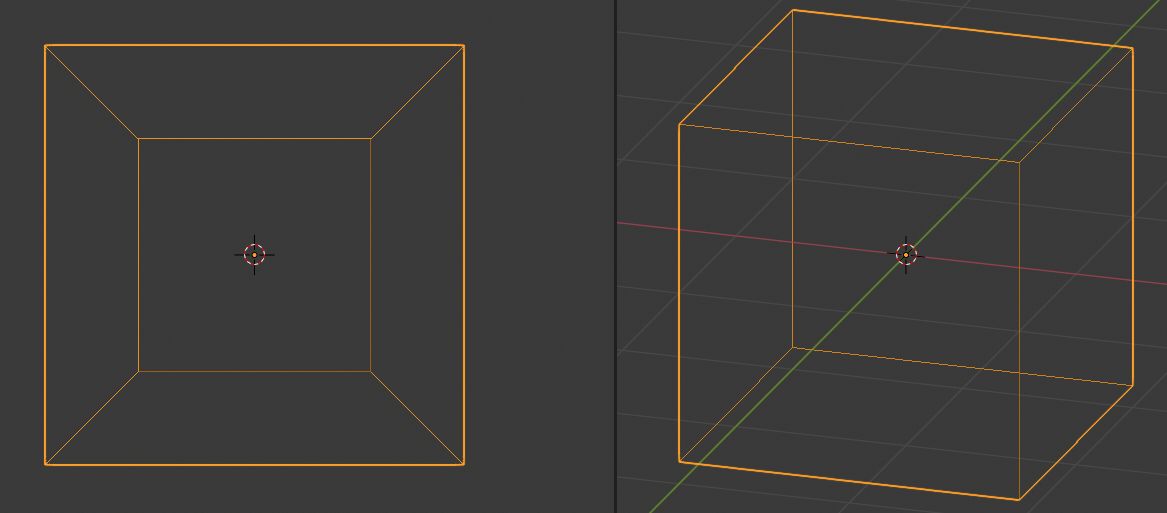
\includegraphics[width=0.5\textwidth]{cube_pespective.PNG}
            \label{fig:enter-label}
        \end{figure}
        \item  Пирамида. Грани разных размеров слиплись в наблюдаемой проекции
        \begin{figure}
            \centering
            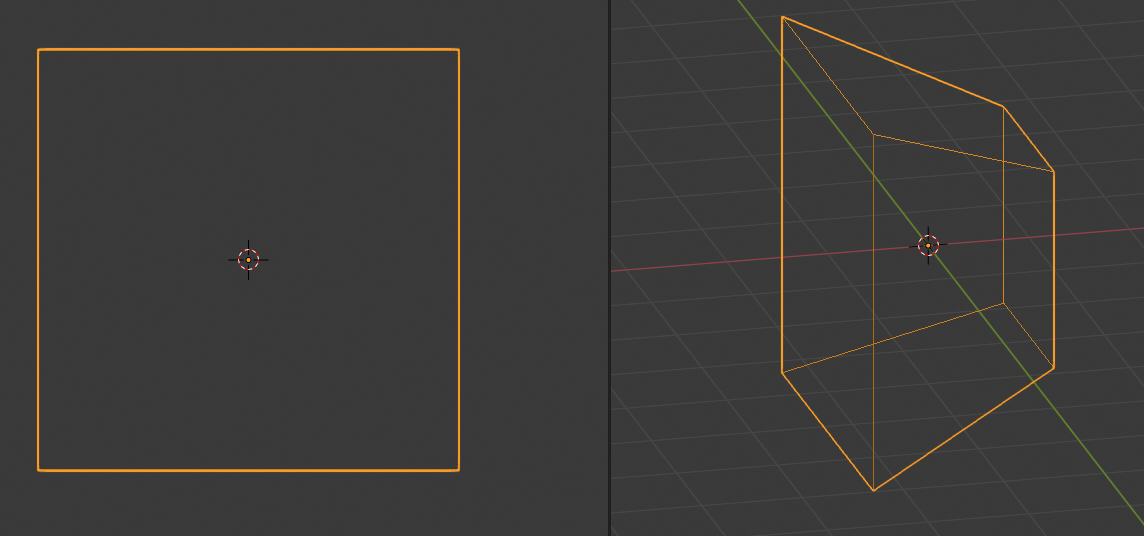
\includegraphics[width=0.5\textwidth]{trapezoid_pespective.PNG}
            \label{fig:enter-label}
        \end{figure}
    \end{itemize}
\end{frame}
\begin{frame}{Гомогенные координаты}
Пусть $X$ --- множество точек, $a = (a_1, a_2, a_3) \in X \setminus \{0\}$. Введем класс эквивалентности $L_a$:
    \begin{equation*}
        L_{a} = \{x \in X \setminus \{0\}: x = \lambda a = (\lambda a_1, \lambda a_2, \lambda a_3),\, \lambda \in \mathcal{R} \}
    \end{equation*}
\begin{alertblock}{Определение}
    В \emph{гомогенных коордианатах} точки, принадлежащие одному и тому же классу эквивалентности $L_{a}$ считаются идентичными.
\end{alertblock}
\begin{block}{Замечание}
    Иногда гомогнные координаты называют \emph{rational coordinates}. Потому что каждая точка в гомогенных определяется не своими координатами, а пропорциями.
\end{block}
\end{frame}

\begin{frame}{Гомогенные координаты в компьютерной графике}
Гомогенные координаты в компьютерной графике реализуются через 4-ю компоненту вектора:
\begin{equation*}
    p_1 = (x, y, z, w) \sim p_0 = (x/w, y/w, z/w, 1)
\end{equation*}
Данное представление позволяет применять как аффинные преобразования, так и преобразования перспективы, используя матричные операции $M \in \mathcal{R}^{4 \times 4}$.
\begin{block}{Замечание}
    Если $w = 0$, то данный объект принято считать за вектор. Поэтому наблюдаем на экране мы только точки, а не вектора!
\end{block}
\end{frame}
\end{document}
